\section{Modello di evoluzione stellare}\label{sec:modello-evoluzione-stellare}

\subsection{Introduzione all'evoluzione stellare}
Data la massa iniziale e la composizione chimica di una data stella, siamo riusciti a costruire un modello che ci permettesse di ottenere una predizione sulla sua luminosità e temperatura. Nella realtà, però, le proprietà di una stella non rimangono costanti nel corso della sua vita, ma variano con il tempo.

Questo processo è principalmente dovuto alla presenza delle reazioni termonucleari all'interno dei vari strati della struttura stellare, le quali si modifica d'intensità e natura durante tutta l'evoluzione della stella, variandone la composizione chimica. Inoltre, dal momento  che la stragrande maggioranza delle strutture cosmiche sono composte da stelle, la radiazione che viene ricevuta deve essere generata principalmente al loro interno. Per capire, quindi, come queste strutture si evolvono è necessario comprendere le varie fasi della vita stellare.

\subsection{Diagramma H-R e traccia evolutiva}

Per avere una rappresentazione visiva dell'evoluzione, costruiamo quello che viene chiamato diagramma di Hertzpsprung-Russell (in breve diagramma H-R) che mostra la dipendenza della luminosità stellare, normalizzata a quella solare, dalla temperatura effettiva %(figura~\ref{fig:HR}).

\begin{figure}
    \centering
    \begin{tikzpicture}
        \begin{axis}[
                title = Diagramma H-R,
                axis x line=center,
                axis y line=center,
                ymin=0, ymax=5,
                xmin=0, xmax=5,
                xlabel = {$-log(T)$},
                ylabel = {$log(\frac{L}{L_\odot})$},
                yticklabels=\empty,
                xticklabels=\empty
        ]
        \end{axis}
    \end{tikzpicture}
    \caption{La figura mostra un diagramma Hertzpsprung-Russell. Si noti che la temperatura, sull'asse delle ascisse, cresce verso sinistra e diminuisce verso destra e che il diagramma è in scala doppio logaritmica.}\label{fig:HR}
\end{figure}

Se il modello stellare considerato precedentemente ha una forma del tipo,
\begin{center}
    \begin{tikzpicture} [
            blu/.style={rectangle, draw=blue!60, fill=blue!5, very thick, minimum size=5mm},
            red/.style={rectangle, draw=red!60, fill=red!5, very thick, minimum size=5mm},
            green/.style={rectangle, draw=green!60, fill=green!5, very thick, minimum size=5mm},]
        \node[red](1){\footnotesize{Massa, X, Y , Z}};
        \node[blu](2)[right=of 1]{\footnotesize{Modello Stellare}};
        \node[green](3)[right=of 2]{\footnotesize{$L, T_e$}};

        \draw[->] (1.east) -- (2.west);
        \draw[->] (2.east) -- (3.west);
    \end{tikzpicture}
\end{center}
quello che definiamo ora contiene una parte dipendente dal tempo:
\begin{center}
    \begin{tikzpicture} [
            blu/.style={rectangle, draw=blue!60, fill=blue!5, very thick, minimum size=5mm},
            red/.style={rectangle, draw=red!60, fill=red!5, very thick, minimum size=5mm},
            green/.style={rectangle, draw=green!60, fill=green!5, very thick, minimum size=5mm},
            black/.style={rectangle, draw=black!60, fill=black!5, very thick, minimum size=5mm},]
        \node[red](1){\footnotesize{Massa, X, Y , Z}};
        \node[black](2)[right=of 1]{\footnotesize{t $+ \Delta$t}};
        \node[blu](3)[right=of 2]{\footnotesize{Modello Stellare}};
        \node[green](4)[right=of 3]{\footnotesize{$L, T_e$}};

        \draw[->] (1.east) -- (2.west);
        \draw[->] (2.east) -- (3.west);
        \draw[->] (3.east) -- (4.west);
    \end{tikzpicture}
\end{center}

Questo perché le reazioni termonucleari all'interno dei una stella bruciano gli elementi più leggeri producendone di più pesanti. Ma non sono tutte reazioni sono uguali, infatti, nel corso dell'evoluzione stellare queste si modificano a seconda del combustibile utilizzato, variando anche la quantità di energia che viene prodotta. Potenzialmente attivando o spegnendo la convezione della stella, o la sua degenerazione.

Tutti questi processi vanno a modificare la luminosità e la temperatura di una stella ed è quindi possibile associare un punto del diagramma H-R per ogni stato di $L$ e $T_e$. In generale, prendendo stelle di masse differenti, ma composizione chimica simile, è possibile costruire un diagramma simile a quello che in cui si osserva l'evoluzione anche in funzione della massa, come mostrato in nella figura~\ref{fig:evo}.
\begin{figure}
    \centering
    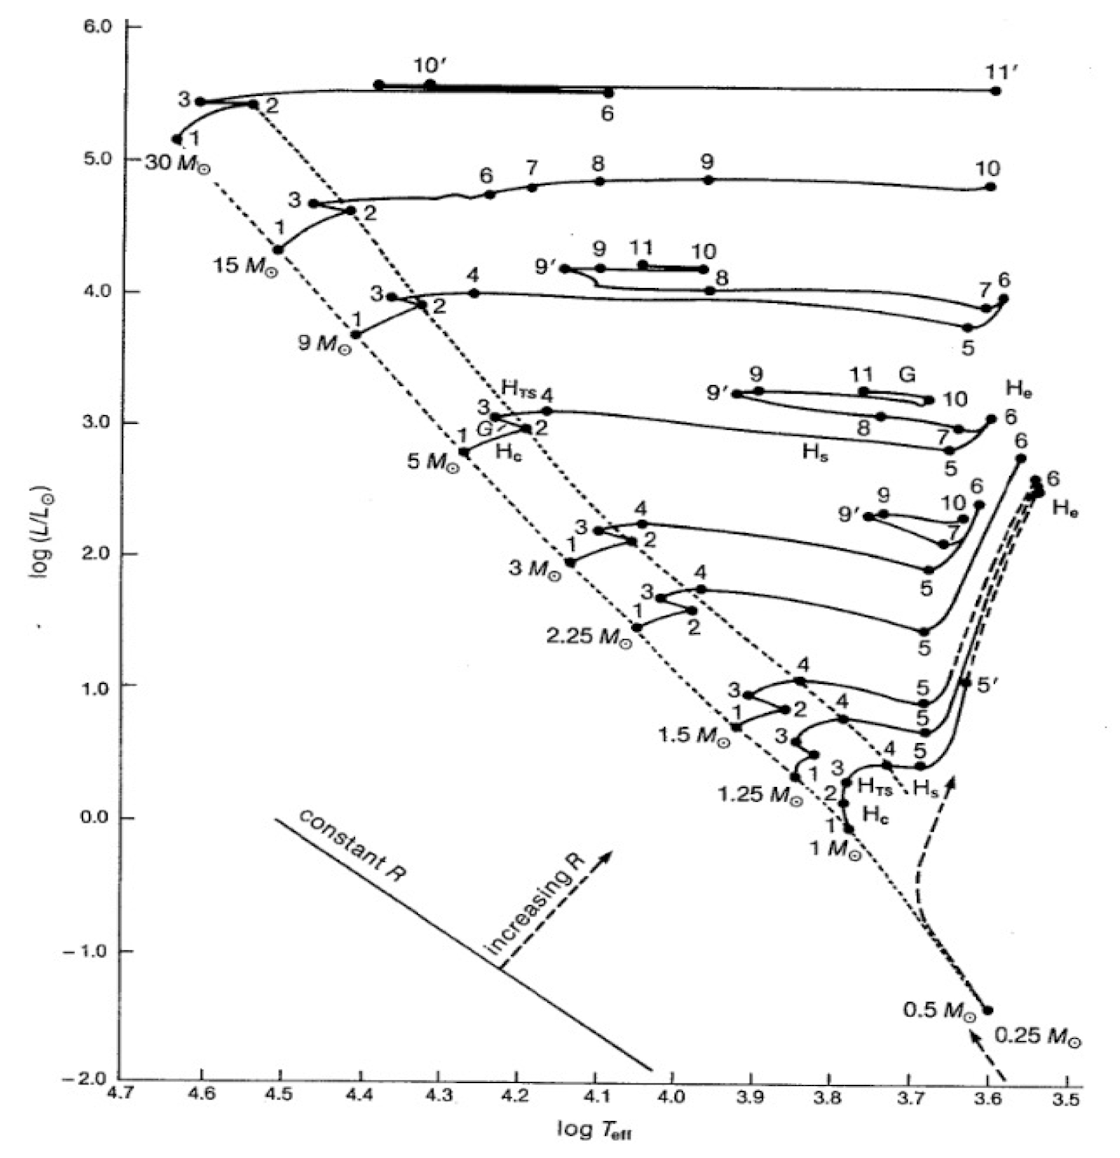
\includegraphics[width=0.5\textwidth]{immagini/evo.png}
    \caption{Nel diagramma H-R sono mostrate nove stelle di massa differente ma di struttura chimica simile evolvere nel tempo.}\label{fig:evo}
\end{figure}